\documentclass[tikz]{standalone}

%inkscape --without-gui --file=ASIL_A.pdf --export-plain-svg=ASIL_A.svg
\usepackage{xcolor}

\begin{document}
	
\begin{tikzpicture}
	\node[draw=black,fill=green] at (0,0) {ASIL A};
	\end{tikzpicture}
	
	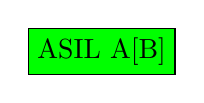
\begin{tikzpicture}
	\node[draw=black,fill=green] at (0,0) {ASIL A[B]};
	\end{tikzpicture}

	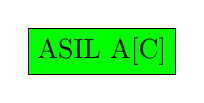
\begin{tikzpicture}
	\node[draw=black,fill=green] at (0,0) {ASIL A[C]};
	\end{tikzpicture}	

	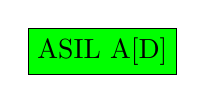
\begin{tikzpicture}
	\node[draw=black,fill=green] at (0,0) {ASIL A[D]};
	\end{tikzpicture}

	
\begin{tikzpicture}
	\node[draw=black,fill=yellow] at (0,0) {ASIL B};
	\end{tikzpicture}
	
	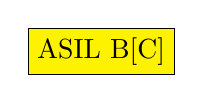
\begin{tikzpicture}
	\node[draw=black,fill=yellow] at (0,0) {ASIL B[C]};
	\end{tikzpicture}	
	
	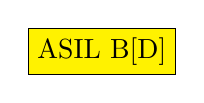
\begin{tikzpicture}
	\node[draw=black,fill=yellow] at (0,0) {ASIL B[D]};
	\end{tikzpicture}
	
	
\begin{tikzpicture}
	\node[draw=black,fill=orange] at (0,0) {ASIL C};
	\end{tikzpicture}
	
	
\begin{tikzpicture}
	\node[draw=black,fill=orange] at (0,0) {ASIL C[D]};
	\end{tikzpicture}
	
	
\begin{tikzpicture}
	\node[draw=black,fill=red] at (0,0) {ASIL D};
	\end{tikzpicture}	
	
	
\begin{tikzpicture}
	\node[draw=black,fill=green] at (0,0) {QM};
	\end{tikzpicture}
	
	
\begin{tikzpicture}
	\node[draw=black,fill=green] at (0,0) {QM[A]};
	\end{tikzpicture}
	
	
\begin{tikzpicture}
	\node[draw=black,fill=green] at (0,0) {QM[B]};
	\end{tikzpicture}					
	
	
\begin{tikzpicture}
	\node[draw=black,fill=green] at (0,0) {QM[C]};
	\end{tikzpicture}		
	
	
\begin{tikzpicture}
	\node[draw=black,fill=green] at (0,0) {QM[D]};
	\end{tikzpicture}	
	
	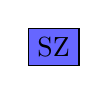
\begin{tikzpicture}
	\node[draw=black,fill=blue!60!white] at (0,0) {SZ};
	\end{tikzpicture}
	
	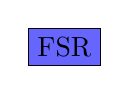
\begin{tikzpicture}
	\node[draw=black,fill=blue!60!white] at (0,0) {FSR};
	\end{tikzpicture}			

	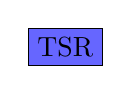
\begin{tikzpicture}
	\node[draw=black,fill=blue!60!white] at (0,0) {TSR};
	\end{tikzpicture}

	
\begin{tikzpicture}
	\node[draw=black,fill=blue!60!white] at (0,0) {Info};
	\end{tikzpicture}
	
	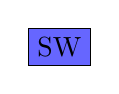
\begin{tikzpicture}
	\node[draw=black,fill=blue!60!white] at (0,0) {SW};
	\end{tikzpicture}
	
	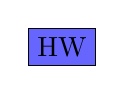
\begin{tikzpicture}
	\node[draw=black,fill=blue!60!white] at (0,0) {HW};
	\end{tikzpicture}	
	
	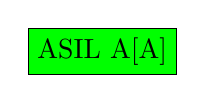
\begin{tikzpicture}
	\node[draw=black,fill=green] at (0,0) {ASIL A[A]};
	\end{tikzpicture}	
	
	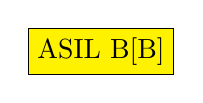
\begin{tikzpicture}
	\node[draw=black,fill=yellow] at (0,0) {ASIL B[B]};
	\end{tikzpicture}	
	
	
\begin{tikzpicture}
	\node[draw=black,fill=orange] at (0,0) {ASIL C[C]};
	\end{tikzpicture}	
	
	
\begin{tikzpicture}
	\node[draw=black,fill=red] at (0,0) {ASIL D[D]};
	\end{tikzpicture}				
\end{document}



